\documentclass{bredelebeamer}

%%%%%%%%%%%%%%%%%%%%%%%%%%%%%%%%%%%%%%%%%%%%%%%%

\title[Programación en MatLAB]{Introducción a la programación con MatLAB}
\subtitle{Módulo 11 - Matemática simbólica}

\author{Autor1 - Autor2 - Autor3\inst{1}}
\institute[UTN.BA]
{
  \inst{1}%
  Universidad Tecnológica Nacional\\
  Facultad Regional Buenos Aires
  }

\date{día mes 2018}

\subject{Taller de programación}

\logo{

\includegraphics[scale=0.15]{images/logo.png}
}

%%%%%%%%%%%%%%%%%%%%%%%%%%%%%%%%%%%%%%%%%%%%%%%%%%%%%%%%%%%%%%%%%%%%%
\begin{document}

\begin{frame}
  \titlepage 
\end{frame}

%%%%%%%%%%%%%%%%%%%%%%%%%%%%%%%%%%%%%%%%%%%%%%%%%%%%%%%%%%%%%%%%%%%%%

% Álgebra matricial

%%%%%%%%%%%%%%%%%%%%%%%%%%%%%%%%%%%%%%%%%%%%%%%%%%%%%%%%%%%%%%%%%%%%%
\section{Matemática simbólica}

\begin{frame}{Introducción}
\begin{center}
\textbf{Con frecuencia es preferible manipular las ecuaciones simbólicamente antes de sustituir valores para las variables.}
\end{center} 
Los objetivos de esta unidad son aprender a:
\begin{itemize}
\item Crear y manipular variables simbólicas
\item Resolver expresiones y ecuaciones simbólicas
\item Graficar ecuaciones simbólicas
\item Introducir al alumno en diferenciación y integración de ecuaciones simbólicas
\end{itemize}
\end{frame}

\begin{frame}{Creación de variables simbólicas}
Existen dos formas posibles de declarar una variable simbólica, las mismas son:
\begin{enumerate}
\item x = sym('x')
\item syms x
\end{enumerate}
\begin{center}
Ambas formas hacen al carácter 'x' igual a la variable simbólica x.
\end{center}
Creación de una variable simbólica utilizando otra existente:
\begin{equation*}
y = \frac{2*(x+3)^2}{x^2+6*x+9}
\end{equation*}
\begin{block}{Tener en cuenta}
El comando \textbf{syms} permite crear múltiples variables simbólicas al mismo tiempo.
\end{block}
\end{frame}

\begin{frame}{Creación de variables simbólicas}
\begin{equation*}
syms x
\end{equation*}
\begin{equation*}
y = \frac{2*(x+3)^2}{x^2+6*x+9}
\end{equation*}
\begin{columns}
\begin{column}{0.5\textwidth}
\begin{center}
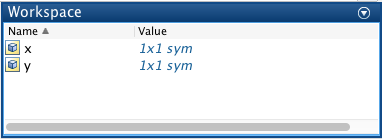
\includegraphics[scale=0.4]{images/fig1.png}
\end{center}
\end{column}
\begin{column}{0.5\textwidth}
\begin{center}
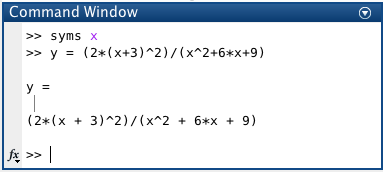
\includegraphics[scale=0.4]{images/fig2.png}
\end{center}
\end{column}
\end{columns}
\end{frame}

\begin{frame}{Manipulación de expresiones y ecuaciones simbólicas}
A continuación, las funciones de manipulación de variables simbólicas se ejemplificarán utilizando la siguiente función:
\begin{equation*}
y = \frac{2*(x+2)^2}{x^2+6*x+9}
\end{equation*}
\end{frame}

\begin{frame}{Manipulación de expresiones y ecuaciones simbólicas}
\begin{center}
Extracción de numeradores y denominadores
\end{center}
\begin{exampleblock}{Comando}
Ver comando: [num,den] = numden(var)
\end{exampleblock}
Ej. Ejecutar las siguientes líneas. Obtener conclusiones.
\boiteviolette{
\begin{equation*}
syms x
\end{equation*}
\begin{equation*}
y = \frac{2*(x+2)^2}{x^2+6*x+9}
\end{equation*}
\begin{equation*}
[num,den] = numden(y)
\end{equation*}
}
\end{frame}

\begin{frame}{Manipulación de expresiones y ecuaciones simbólicas}
\begin{center}
Expansión de expresiones\\
\textit{(Multiplica todas las porciones de la ecuación)}
\end{center}
\begin{exampleblock}{Comando}
Ver comando: expand(var)
\end{exampleblock}
Ej. Ejecutar las siguientes líneas. Obtener conclusiones.
\boiteviolette{
\begin{equation*}
syms x
\end{equation*}
\begin{equation*}
y = \frac{2*(x+2)^2}{x^2+6*x+9}
\end{equation*}
\begin{equation*}
[num,den] = numden(y)
\end{equation*}
\begin{equation*}
expand(num)
\end{equation*}
}
\end{frame}

\begin{frame}{Manipulación de expresiones y ecuaciones simbólicas}
\begin{center}
Factorización de expresiones\\
\textit{(Factoriza la ecuación)}
\end{center}
\begin{exampleblock}{Comando}
Ver comando: factor(var)
\end{exampleblock}
Ej. Ejecutar las siguientes líneas. Obtener conclusiones.
\boiteviolette{
\begin{equation*}
syms x
\end{equation*}
\begin{equation*}
y = \frac{2*(x+2)^2}{x^2+6*x+9}
\end{equation*}
\begin{equation*}
[num,den] = numden(y)
\end{equation*}
\begin{equation*}
factor(num)
\end{equation*}
}
\end{frame}

\begin{frame}{Manipulación de expresiones y ecuaciones simbólicas}
\begin{center}
Recolección de términos\\
\textit{(Recopila términos similares)}
\end{center}
\begin{exampleblock}{Comando}
Ver comando: collect(var)
\end{exampleblock}
Ej. Ejecutar las siguientes líneas. Obtener conclusiones.
\boiteviolette{
\begin{equation*}
syms x
\end{equation*}
\begin{equation*}
y = \frac{2*(x+2)^2}{x^2+6*x+9}
\end{equation*}
\begin{equation*}
[num,den] = numden(y)
\end{equation*}
\begin{equation*}
collect(num)
\end{equation*}
}
\end{frame}

\begin{frame}{Simplificación de ecuaciones simbólicas}
\begin{exampleblock}{Comando}
Ver comando: simplify(var)
\end{exampleblock}
Ej. Ejecutar las siguientes líneas. Obtener conclusiones.
\boiteviolette{
\begin{equation*}
z = sym('x^3-1=(x-3)*(x+3)') 
\end{equation*}
\begin{equation*}
simplify(z)
\end{equation*}
}
\end{frame}

\begin{frame}{Ejercicio práctico xxx}
\begin{enumerate}
\item Cree las variables simbólicas x,a,b,c y d
\item Verifique que las variables creadas en el item (1) se mencionan en la ventana del área de trabajo. Úselas para crear las siguientes expresiones simbólicas:
\begin{itemize}
\item $ex1 = x^2-1$
\item $ex2 = (x+1)^2$
\item $ex3 = a*x^2-1$
\item $ex4 = a*x^2+b*x+c$
\item $ex5 = a*x^3+b*x^2+c*x+d$
\end{itemize}
\item Multiplique ex1 por ex2 y llame al resultado y1
\item Divida ex1 entre ex2 y llame al resultado y2
\item Use la función numden para extraer el numerador y denominador de y1 y y2
\item Use las funciones factor, expand, collect y simplify en y1 e y2.\\Obtenga conclusiones.
\end{enumerate}
\end{frame}

\begin{frame}{Sugerencia}
Para crear un polinomio simbólico a partir de un vector de números se utiliza la función \textbf{poly2sym}
\begin{exampleblock}{Comando}
Ver comando: poly2sym()
\end{exampleblock}
Ej. Ejecutar las siguientes líneas. Obtener conclusiones.
\boiteviolette{
\begin{equation*}
a = [1 3 2]
\end{equation*}
\begin{equation*}
b = poly2sym(a)
\end{equation*}
}
De modo similar, \textbf{sym2poly} convierte un polinomio en un vector de valores.
\begin{exampleblock}{Comando}
Ver comando: sym2poly()
\end{exampleblock}
\end{frame}

\begin{frame}{Resolución de expresiones y ecuaciones simbólicas}
Para la resolución de expresiones y ecuaciones (dos expresiones igualadas) se utilizará la función solve.
\begin{exampleblock}{Comando}
Ver comando: solve()
\end{exampleblock}
Se utilizarán dos enfoques, los mismos son:
\begin{enumerate}
\item Cuando se trata de una expresión
\item Cuando se trata de una ecuación
\begin{enumerate}
\item Expresión igualada a 0
\item Expresión igualada a una expresión distinta de 0 (aplicando transformación)
\item Expresión igualada a una expresión distinta de 0 (sin transformación)
\end{enumerate}
\end{enumerate}
\end{frame}

\begin{frame}{Resolución de expresiones y ecuaciones simbólicas: Caso 1}
\begin{center}
Utilización de la función \textbf{solve} en una expresión
\end{center}
Ej. Ejecutar las siguientes líneas. Obtener conclusiones.
\boiteviolette{
\begin{equation*}
E1 = x-3 
\end{equation*}
\begin{equation*}
solve(E1)
\end{equation*}
}
\begin{alertblock}{Importante}
Cuando se usa en una expresión, la función \textbf{solve} iguala la expresión a cero y resuelve.
\end{alertblock}
\end{frame}

\begin{frame}{Resolución de expresiones y ecuaciones simbólicas: Caso 1}
Ej. Ejecutar las siguientes líneas. Obtener conclusiones.
\boiteviolette{
\begin{equation*}
solve('a*x^2+b*x+c')
\end{equation*}
}
\begin{alertblock}{Importante}
Matlab por defecto resuelve para la variable simbólica x. 
\end{alertblock}
\end{frame}

\begin{frame}{Resolución de expresiones y ecuaciones simbólicas: Caso 1}
Para el caso en que se desee especificar la variable por resolver, ésta debe ser indicada en el segundo campo de la función.\\
Ej. Ejecutar las siguientes líneas. Obtener conclusiones.
\boiteviolette{
\begin{equation*}
solve('a*x^2+b*x+c','a')
\end{equation*}
}
\begin{block}{Tener en cuenta}
Si \textbf{a} se define específicamente como variable simbólica, no es necesaria encerrarla entre apóstrofes.
\end{block}
\end{frame}

\begin{frame}{Resolución de expresiones y ecuaciones simbólicas: Caso 2.1 ó 2.2}
Si la ecuación es simple, puede transformarse en una expresión al restar el lado derecho del lado izquierdo.\\
Para el caso:
\begin{equation*}
5*x^2+6*x+3=10
\end{equation*}
Se podría reformular como:
\begin{equation*}
5*x^2+6*x-7=0
\end{equation*}
y resolver la ecuación ejecutando las siguientes líneas:
\boiteviolette{
\begin{equation*}
solve('5*x^2+6*x-7') 
\end{equation*}
}
\end{frame}

\begin{frame}{Resolución de expresiones y ecuaciones simbólicas: Caso 2.3}
Si la ecuación es compleja, se define una nueva ecuación y luego se procede a resolver la misma.
Para el caso:
\begin{equation*}
5*x^2+6*x+3=10
\end{equation*}

Se resuelve la ecuación ejecutando las siguientes líneas:
\boiteviolette{
\begin{equation*}
E2 = sym('5*x^2+6*x+3=10') 
\end{equation*}
\begin{equation*}
solve(E2) 
\end{equation*}
}
\end{frame}

\begin{frame}{Ejercicio práctico xxx}
\begin{enumerate}
\item Cree las variables simbólicas x,a,b,c y d
\item Verifique que las variables creadas en el item (1) se mencionan en la ventana del área de trabajo. Úselas para crear las siguientes expresiones simbólicas:
\begin{itemize}
\item $ex1 = x^2-1$
\item $ex2 = (x+1)^2$
\item $ex3 = a*x^2-1$
\item $ex4 = a*x^2+b*x+c$
\item $ex5 = a*x^3+b*x^2+c*x+d$
\end{itemize}
\begin{itemize}
\item $eq1 = x^2=1$
\item $eq2 = (x+1)^2=0$
\item $eq3 = a*x^2=1$
\item $eq4 = a*x^2+b*x+c=0$
\item $eq5 = a*x^3+b*x^2+c*x+d=0$
\end{itemize}
\item Use la función solve para resolver ex1 y eq1
\item Use la función solve para resolver ex2 y eq2
\item Use la función solve para resolver ex3 y eq3 tanto para x como para a
\item Use la función solve para resolver ex4 y eq4 tanto para x como para a
\end{enumerate}
\end{frame}

\begin{frame}{Resolución de sistemas de ecuaciones}
Se desea resolver el siguiente sistemas de ecuaciones utilizando la función \textbf{solve}:
\begin{equation*}
\left\{\begin{matrix}
3x + 2y - z = 10  \\ 
-x +3y +2z = 5  \\ 
 x - y - z = -1 
\end{matrix}\right.
\end{equation*}
\end{frame}

\begin{frame}{Resolución de sistemas de ecuaciones}
\begin{itemize}
\item Definir las tres ecuaciones simbólicas
\end{itemize}
\begin{equation*}
Ec1 = sym('3*x+2*y-z=10')
\end{equation*}
\begin{equation*}
Ec2 = sym('-x+3*y+2*z=5')
\end{equation*}
\begin{equation*}
Ec3 = sym('x-y-z=-1')
\end{equation*}
Luego utilizando la función \textbf{solve} se obtienen la solución (valores de x, y, z):
\boiteviolette{
\begin{center}
[x,y,z] = solve(Ec1,Ec2,Ec3)
\end{center}
}
\end{frame}

\begin{frame}{Graficación de ecuaciones simbólicas}
Se realizará la gráfica de una función de la forma:
\begin{center}
\begin{equation*}
y = f(x)
\end{equation*}
\end{center}
\begin{exampleblock}{Comando}
Ver comando: ezplot()
\end{exampleblock}
Ej. Ejecutar las siguientes líneas. Obtener conclusiones.
\boiteviolette{
\begin{equation*}
y = sym('x^2-2') 
\end{equation*}
\begin{equation*}
ezplot(y)
\end{equation*}
}
\begin{alertblock}{Importante}
Por defecto, se grafica la función con una variación de x en el intervalo $[-2*\pi ,2*\pi ]$
\end{alertblock}
\end{frame}

\begin{frame}{Graficación de ecuaciones simbólicas}
Ej. Ejecutar las siguientes líneas. Obtener conclusiones.
\boiteviolette{
\begin{equation*}
y = sym('x^2-2') 
\end{equation*}
\begin{equation*}
ezplot(y,[-10,10])
\end{equation*}
}
\begin{center}
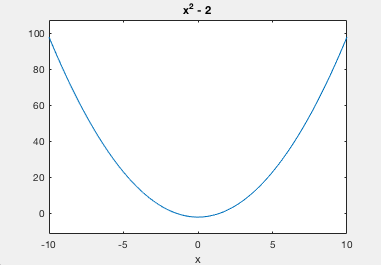
\includegraphics[scale=0.4]{images/fig3.png}
\end{center}
\end{frame}

\begin{frame}{Graficación de ecuaciones simbólicas}
Para graficar una ecuación paramétrica se define ecuaciones separadas para x e y en términos de una tercera variable. Luego se utiliza la función \textbf{ezplot} vista.
\begin{center}
\begin{equation*}
x = sen(t)
\end{equation*}
\begin{equation*}
y = cos(t)
\end{equation*}
\end{center}
Ej. Ejecutar las siguientes líneas. Obtener conclusiones.
\boiteviolette{
\begin{equation*}
ezplot('sin(x)','cos(x)') 
\end{equation*}
}
\begin{center}
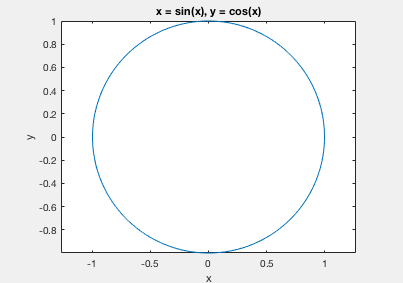
\includegraphics[scale=0.3]{images/fig4.png}
\end{center}
\end{frame}

\begin{frame}{Graficación de ecuaciones simbólicas}
\begin{center}
\begin{equation*}
y_1 = sym('sen(X)') 
\end{equation*}
\begin{equation*}
y_2 = sym('sen(2*X)') 
\end{equation*}
\begin{equation*}
y_3 = sym('sen(3*X)') 
\end{equation*}
\end{center}
Ej. Ejecutar las siguientes líneas. Obtener conclusiones.
\boiteviolette{
\begin{equation*}
ezplot(y_1)
hold on
\end{equation*}
}
\begin{center}
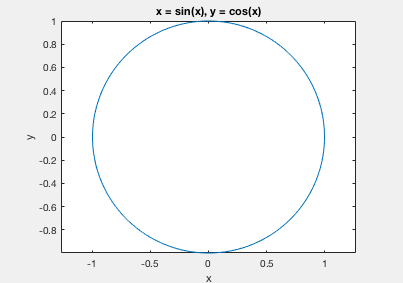
\includegraphics[scale=0.3]{images/fig4.png}
\end{center}
\end{frame}

\begin{frame}{Graficación de ecuaciones simbólicas}
\begin{center}
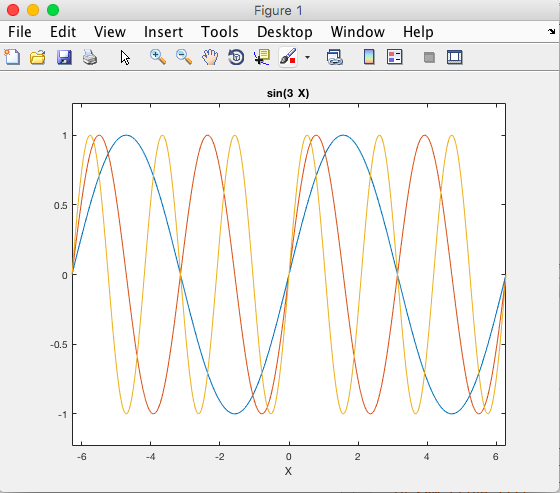
\includegraphics[scale=0.35]{images/fig5.png}
\end{center}
\end{frame}

\begin{frame}{Cálculo: Introducción a la diferenciación}
Se considera un auto de carreras cuya ecuación de posición es:
\begin{equation*}
d=20+20*sen(\frac{\pi *(t-10))}{20})
\end{equation*}
\begin{columns}
\begin{column}{0.5\textwidth}
\boiteviolette{
\begin{equation*}
dist = sym('20+20*sin(\pi *(t-10)/20)')
\end{equation*}
\begin{equation*}
ezplot(dist,[0,20])
\end{equation*}
\begin{equation*}
title('Posición del auto')
\end{equation*}
\begin{equation*}
xlabel('Tiempo [s]')
\end{equation*}
\begin{equation*}
ylabel('Distancia desde la línea de partida') 
\end{equation*}
}
\end{column}
\begin{column}{0.5\textwidth}
\begin{center}
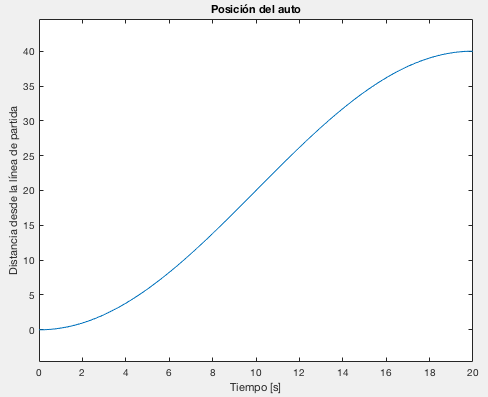
\includegraphics[scale=0.3]{images/fig6.png}
\end{center}
\end{column}
\end{columns}
\end{frame}

\begin{frame}{Cálculo: Introducción a la diferenciación}
Sabiendo que la velocidad es la derivada de la posiócin y utilizando la función \textbf{diff}
\begin{exampleblock}{Comando}
Ver comando: diff()
\end{exampleblock}
Se obtiene la siguiente curva de velocidad
\begin{columns}
\begin{column}{0.5\textwidth}
\boiteviolette{
\begin{equation*}
vel = diff(dist)
\end{equation*}
\begin{equation*}
ezplot(vel,[0,20])
\end{equation*}
\begin{equation*}
title('Velocidad del auto')
\end{equation*}
\begin{equation*}
xlabel('Tiempo [s]')
\end{equation*}
\begin{equation*}
ylabel('Velocidad del auto') 
\end{equation*}
}
\end{column}
\begin{column}{0.5\textwidth}
\begin{center}
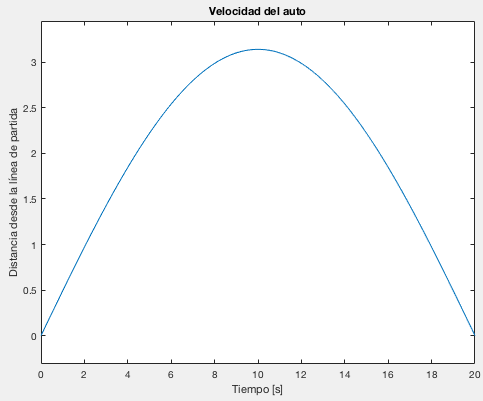
\includegraphics[scale=0.3]{images/fig7.png}
\end{center}
\end{column}
\end{columns}
\end{frame}

\begin{frame}{Cálculo: Introducción a la diferenciación}
Sabiendo que la aceleración es la derivada de la velocidad y utilizando la función \textbf{diff}
\begin{exampleblock}{Comando}
Ver comando: diff()
\end{exampleblock}
Se obtiene la siguiente curva de aceleración
\begin{columns}
\begin{column}{0.5\textwidth}
\boiteviolette{
\begin{equation*}
ace = diff(vel)
\end{equation*}
\begin{equation*}
ezplot(ace,[0,20])
\end{equation*}
\begin{equation*}
title('Aceleración del auto')
\end{equation*}
\begin{equation*}
xlabel('Tiempo [s]')
\end{equation*}
\begin{equation*}
ylabel('Aceleración del auto') 
\end{equation*}
}
\end{column}
\begin{column}{0.5\textwidth}
\begin{center}
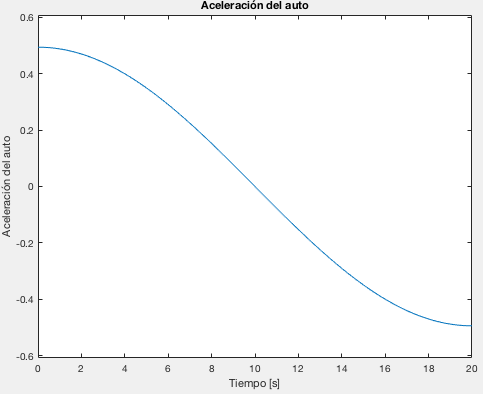
\includegraphics[scale=0.3]{images/fig8.png}
\end{center}
\end{column}
\end{columns}
\end{frame}

\begin{frame}{Cálculo: Introducción a la diferenciación}
\begin{center}
Otras funciones de diferenciación simbólica
\end{center}
\begin{table}[]
\centering
\begin{tabular}{|c|c|}
\hline
diff(f)       & Derivada de la expresión f con respecto a la variable independiente     \\ \hline
diff(f,'t')   & Derivada de la expresión f con respecto a la variable t                 \\ \hline
diff(f,n)     & Derivada n-ésima de la expresión f respecto a la variable independeinte \\ \hline
diff(f,'t',n) & Derivada n-ésima de la expresión f respecto a la variable t             \\ \hline
\end{tabular}
\end{table}
\end{frame}

\begin{frame}{Ejercicio práctico xxx}
\begin{enumerate}
\item Encuentre la primera derivada con respecto a x de las siguientes expresiones:
\begin{enumerate}
\item $x^2+x+1$
\item $sen(x)$
\item $tan(X)$
\item $ln(x)$
\end{enumerate}
\item Encuentre la primera derivada parcial con respecto a x de las siguientes expresiones:
\begin{enumerate}
\item $a*X+b*x+c$
\item $x^0.5 -3*y$
\item $tan(x+y)$
\item $3*x+4*y-3*x*y$
\end{enumerate}
\item Encuentre la segunda derivada con respecto a x para cada una de las expresiones del problema 1 y 2.
\item Encuentre la primera derivada con respecto a y para las siguientes expresiones:
\begin{enumerate}
\item $y-1$
\item $2*y+3*x^2$
\item $a*y+b*x+c*z$
\end{enumerate}
\end{enumerate}
\end{frame}

\begin{frame}{Cálculo: Introducción a la integración}
Dada la curva de aceleración vista, se procede a calcular la velocidad integrando la misma. 
\begin{exampleblock}{Comando}
Ver comando: int()
\end{exampleblock}
Se obtiene la siguiente curva de velocidad
\begin{columns}
\begin{column}{0.5\textwidth}
\boiteviolette{
\begin{equation*}
vel = int(ace)
\end{equation*}
\begin{equation*}
ezplot(vel,[0,20])
\end{equation*}
\begin{equation*}
title('Velocidad del auto')
\end{equation*}
\begin{equation*}
xlabel('Tiempo [s]')
\end{equation*}
\begin{equation*}
ylabel('Velocidad del auto') 
\end{equation*}
}
\end{column}
\begin{column}{0.5\textwidth}
\begin{center}
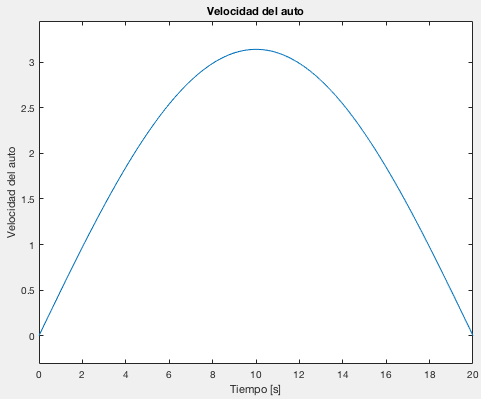
\includegraphics[scale=0.3]{images/fig9.png}
\end{center}
\end{column}
\end{columns}
\end{frame}

\begin{frame}{Cálculo: Introducción a la integración}
Si se desea calcular la integral definida se debe especificar el rango de interés. Algunas funciones para el cálculo de integral numérica son:
\begin{table}[]
\centering
\begin{tabular}{|c|c|}
\hline
int(f)     & Integral de la expresión f con respecto a la variable independiente                                                                      \\ \hline
int(f,'t') & Integral de la expresión f con respecto a la variable t                                                                                  \\ \hline
int(f,a,b) & \begin{tabular}[c]{@{}c@{}}Integral con respecto a la variable independiente de la expresión f \\ entre las fronteras a y b\end{tabular} \\ \hline
\end{tabular}
\end{table}
\end{frame}

\begin{frame}{Ejercicio práctico xxx}
\begin{enumerate}
\item Integre las siguientes expresiones con respecto a x:
\begin{enumerate}
\item $x^2+x+1$
\item $sen(x)$
\item $tan(X)$
\item $ln(x)$
\end{enumerate}
\item Integre las siguientes expresiones con respecto a x:
\begin{enumerate}
\item $a*X+b*x+c$
\item $x^0.5 -3*y$
\item $tan(x+y)$
\item $3*x+4*y-3*x*y$
\end{enumerate}
\item Realice una integración doble con respecto a x para cada una de las expresiones de los problemas 1 y 2.
\item Integre las siguientes expresiones con respecto a y:
\begin{enumerate}
\item $y-1$
\item $2*y+3*x^2$
\item $a*y+b*x+c*z$
\end{enumerate}
\end{enumerate}
\end{frame}


%%%%%%%%%%%%%%%%%%%%%%%%%%%%%%%%%%%%%%%%%%%%%%%%%%%%%%%%%%%%%%%%%%%%%

% Sección de consultas

%%%%%%%%%%%%%%%%%%%%%%%%%%%%%%%%%%%%%%%%%%%%%%%%%%%%%%%%%%%%%%%%%%%%%

\section{Consultas}
\begin{frame}{Consultas}
\begin{center}

\includegraphics[scale=0.3]{images/consultas.png}
\end{center}
\end{frame}


%%%%%%%%%%%%%%%%%%%%%%%%%%%%%%%%%%%%%%%%%%%%%%%%%%%%%%%%%%%%%%%%%%%%%

% Sección de bibliografía

%%%%%%%%%%%%%%%%%%%%%%%%%%%%%%%%%%%%%%%%%%%%%%%%%%%%%%%%%%%%%%%%%%%%%

\section{Bibliografia}

\begin{frame}{Bibliografía}
\begin{columns}
\begin{column}{0.5\textwidth}
\begin{center}

\includegraphics[scale=0.4]{images/biblio1.png}
\end{center}
\end{column}
\begin{column}{0.5\textwidth}
\begin{center}
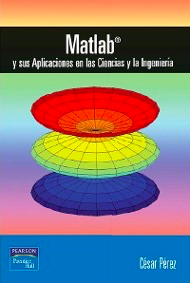
\includegraphics[scale=0.5]{images/biblio2.png}
\end{center}
\end{column}
\end{columns}
\end{frame}

\end{document}
